\documentclass[tikz,border=6pt]{standalone}
\usepackage[T1]{fontenc}
\usepackage{lmodern}
\usepackage{amsmath,amssymb}
\usetikzlibrary{positioning,arrows.meta,fit,calc}
% Design of koblitz-n83-knownlog-20261019 (frozen protocol.json). Not a result.
\begin{document}
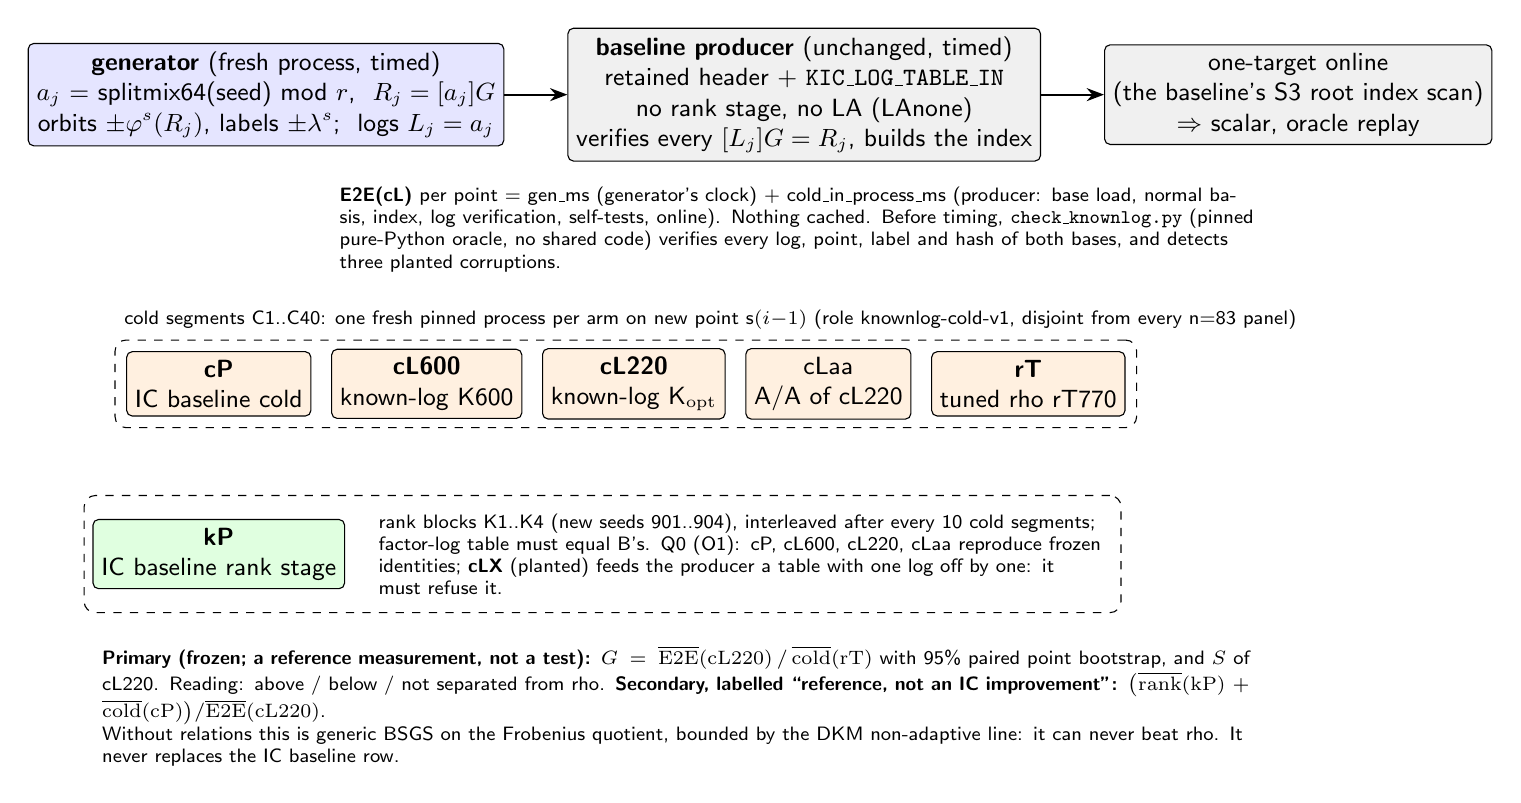
\begin{tikzpicture}[
  font=\sffamily\small,
  box/.style={draw, rounded corners=2pt, align=center, minimum height=8mm, inner sep=3pt},
  base/.style={box, fill=gray!12},
  add/.style={box, fill=blue!10},
  arm/.style={box, fill=orange!12, minimum width=19mm},
  rank/.style={box, fill=green!12, minimum width=19mm},
  arr/.style={-{Stealth[length=2.2mm]}, thick},
  note/.style={align=left, font=\sffamily\scriptsize}
]
% Pipeline of one known-log process
\node[add] (gen) {\textbf{generator} (fresh process, timed)\\$a_j$ = splitmix64(seed) mod $r$, \ $R_j=[a_j]G$\\orbits $\pm\varphi^s(R_j)$, labels $\pm\lambda^s$; \ logs $L_j=a_j$};
\node[base, right=8mm of gen] (prod) {\textbf{baseline producer} (unchanged, timed)\\retained header + \texttt{KIC\_LOG\_TABLE\_IN}\\no rank stage, no LA (\textsf{LAnone})\\verifies every $[L_j]G=R_j$, builds the index};
\node[base, right=8mm of prod] (on) {one-target online\\(the baseline's S3 root index scan)\\$\Rightarrow$ scalar, oracle replay};
\draw[arr] (gen) -- (prod); \draw[arr] (prod) -- (on);
\node[note, below=2mm of prod, text width=118mm] (e2e) {\textbf{E2E(cL)} per point = gen\_ms (generator's clock) + cold\_in\_process\_ms (producer: base load, normal basis, index, log verification, self-tests, online). Nothing cached.
Before timing, \texttt{check\_knownlog.py} (pinned pure-Python oracle, no shared code) verifies every log, point, label and hash of both bases, and detects three planted corruptions.};

% Cold arms
\node[arm, below=26mm of gen, xshift=-6mm] (cP) {\textbf{cP}\\IC baseline cold};
\node[arm, right=2.5mm of cP] (c600) {\textbf{cL600}\\known-log K600};
\node[arm, right=2.5mm of c600] (c220) {\textbf{cL220}\\known-log K$_\mathrm{opt}$};
\node[arm, right=2.5mm of c220] (caa) {cLaa\\A/A of cL220};
\node[arm, right=2.5mm of caa] (rT) {\textbf{rT}\\tuned rho rT770};
\node[draw, dashed, rounded corners, fit=(cP) (rT), inner sep=4pt, label={[note, anchor=south west]north west:{cold segments C1..C40: one fresh pinned process per arm on new point s$(i{-}1)$ (role knownlog-cold-v1, disjoint from every n=83 panel)}}] (cold) {};
\node[rank, below=13mm of cP] (kP) {\textbf{kP}\\IC baseline rank stage};
\node[note, right=3mm of kP, text width=92mm] (kb) {rank blocks K1..K4 (new seeds 901..904), interleaved after every 10 cold segments; factor-log table must equal B's.
Q0 (O1): cP, cL600, cL220, cLaa reproduce frozen identities; \textbf{cLX} (planted) feeds the producer a table with one log off by one: it must refuse it.};
\node[draw, dashed, rounded corners, fit=(kP) (kb), inner sep=3pt] {};

\node[note, anchor=north west, text width=150mm] (eq) at ($(kP.south west)+(0,-6mm)$) {\textbf{Primary (frozen; a reference measurement, not a test):}
$G=\overline{\mathrm{E2E}}(\mathrm{cL220})\,/\,\overline{\mathrm{cold}}(\mathrm{rT})$ with 95\% paired point bootstrap, and $S$ of cL220.
Reading: above / below / not separated from rho.
\textbf{Secondary, labelled ``reference, not an IC improvement'':} $\big(\overline{\mathrm{rank}}(\mathrm{kP})+\overline{\mathrm{cold}}(\mathrm{cP})\big)/\overline{\mathrm{E2E}}(\mathrm{cL220})$.\\
Without relations this is generic BSGS on the Frobenius quotient, bounded by the DKM non-adaptive line: it can never beat rho. It never replaces the IC baseline row.};
\end{tikzpicture}
\end{document}
